% !TeX program = pdflatex
% =============================================================================
% Experimente 1: Kraftaddition & Kraftzerlegung
% UZH Praktikum I -- Sara Romer Urban, Kantonsschule im Lee, HS2026
% Klasse: 2e (02.09.2026)
%
% Sammlung kurzer Demoversuche zur Doppellektion Kraftaddition/-zerlegung,
% als Ergaenzung zu kraefte-addieren-zerlegen-lektionsplan.tex (nicht Ersatz
% fuer das Arbeitsblatt/Aufgabenblatt). Zwei Versuche: (1) Faden zwischen
% zwei Stangen mit wenig Durchhang gespannt, reisst beim Anhaengen einer
% Masse -- derselbe Grenzfall-Gedanke wie in Aufgabenblatt 2, Aufgabe 5
% (kleiner Winkel -> riesige Seilspannkraft), hier aber als reales
% Tischexperiment statt als Konstruktionsaufgabe. (2) Klassischer
% Tischrand-Versuch mit zwei Maennchen, deren Nasen ueber ein an der
% Tischkante umgelenktes Seil mit einem haengenden Gewicht verbunden sind --
% zeigt, wie sich eine konstante Seilkraft mit wachsendem Winkel von
% horizontal (ziehend) zu vertikal (hebend) verlagert.
% =============================================================================
\documentclass[11pt,a4paper]{article}

\usepackage[T1]{fontenc}
\usepackage[utf8]{inputenc}
\usepackage[ngerman]{babel}
\usepackage{lmodern}
\usepackage[a4paper,margin=2.2cm]{geometry}
\usepackage{amsmath}
\usepackage{siunitx}
\sisetup{per-mode=fraction,fraction-command=\frac}
\usepackage{xcolor}
\usepackage{tikz}
\usepackage{graphicx}
\usetikzlibrary{arrows.meta,calc}

\definecolor{titleblue}{HTML}{183A6B}
\definecolor{accentorange}{HTML}{D9720C}
\definecolor{darkgray}{HTML}{4A4A4A}
\definecolor{warnred}{HTML}{9E2E2E}

\setlength{\parindent}{0pt}
\setlength{\parskip}{0.6em}

\usepackage{titlesec}
\titleformat{\section}{\Large\bfseries\color{titleblue}}{\thesection}{0.6em}{}
\titlespacing*{\section}{0pt}{1.2em}{0.5em}

\begin{document}
\sloppy

\begin{center}
{\Huge\bfseries\color{titleblue}Experimente 1: Kraftaddition \& Kraftzerlegung}\\[0.4em]
{\large Kurze Demoversuche zur Doppellektion}
\end{center}
\vspace{0.5em}

\noindent\textbf{Klasse:} 2e (02.09.2026) \hfill \textbf{Lehrperson:} Loris Keller

\vspace{0.3em}
\noindent\textcolor{darkgray}{Dieses Dokument sammelt kurze Demoversuche zur
Doppellektion Kraftaddition \& Kraftzerlegung, mit Skizze und kurzer
Erklärung pro Versuch, als Ergänzung zum Unterricht, nicht als Ersatz für
Arbeitsblatt oder Aufgabenblatt.}

% =============================================================================
\section*{Experiment 1: Warum reisst der Faden?}

\textbf{Aufbau:} Ein dünner Faden wird zwischen zwei Stangen befestigt und
so gespannt, dass er nur ganz wenig durchhängt (kleiner Winkel zur
Horizontalen). Anschliessend wird in der Mitte eine Masse an den Faden
gehängt, und der Faden reisst.

\begin{center}
\begin{tikzpicture}[>=Latex,scale=1.15]
  \draw[very thick,darkgray] (-3,0) -- (-3,3);
  \draw[very thick,darkgray] (3,0) -- (3,3);
  \draw[thick,darkgray] (-3,3) -- (3,3);
  \node[below] at (0,-0.3) {\small Vorher: Faden gespannt, kaum Durchhang};
\end{tikzpicture}
\hspace{1cm}
\begin{tikzpicture}[>=Latex,scale=1.15]
  \draw[very thick,darkgray] (-3,0) -- (-3,3);
  \draw[very thick,darkgray] (3,0) -- (3,3);
  \draw[thick,darkgray] (-3,3) -- (-0.3,2.85);
  \draw[thick,darkgray] (0.3,2.85) -- (3,3);
  \draw[thick,warnred] (-0.3,2.85) -- (-0.15,2.65) -- (0,2.9) -- (0.15,2.6) -- (0.3,2.85);
  \draw[->,thick,accentorange] (0,2.3) -- (0,1.3);
  \filldraw[darkgray] (0,1.9) circle (0.22);
  \node[right] at (0.4,1.6) {\small Masse fällt};
  \node[below] at (0,-0.3) {\small Nachher: Masse angehängt, Faden reisst};
\end{tikzpicture}
\end{center}

\textbf{Erklärung:} Solange der Faden fast gerade gespannt ist, bildet er
mit der Horizontalen nur einen sehr kleinen Winkel. Genau wie bei der
Lampe in Aufgabenblatt 2, Aufgabe 5 gilt: Je kleiner dieser Winkel, desto
länger müssten die beiden Fadenspannkräfte beim Kräfteparallelogramm
gezeichnet werden, um zusammen die Gewichtskraft der angehängten Masse zu
tragen. Die nötige Spannkraft im Faden wird also riesig gross. Ein
dünner Faden hält aber nur eine begrenzte Kraft aus, bevor er reisst.
Deshalb genügt schon eine kleine Masse, um den fast straff gespannten
Faden zum Reissen zu bringen.

% =============================================================================
\section*{Experiment 2: Männchen am Tischrand}

\textbf{Aufbau:} Zwei Männchen stehen auf dem Tisch. Ihre Nasen sind über
ein Seil, das an der Tischkante umgelenkt wird, mit einem Gewicht
verbunden, das über den Tischrand hinunterhängt. Das Gewicht zieht die
Männchen an der Nase Schritt für Schritt Richtung Tischrand, bis sie
schliesslich anhalten, kurz bevor sie den Rand erreichen.

\begin{center}
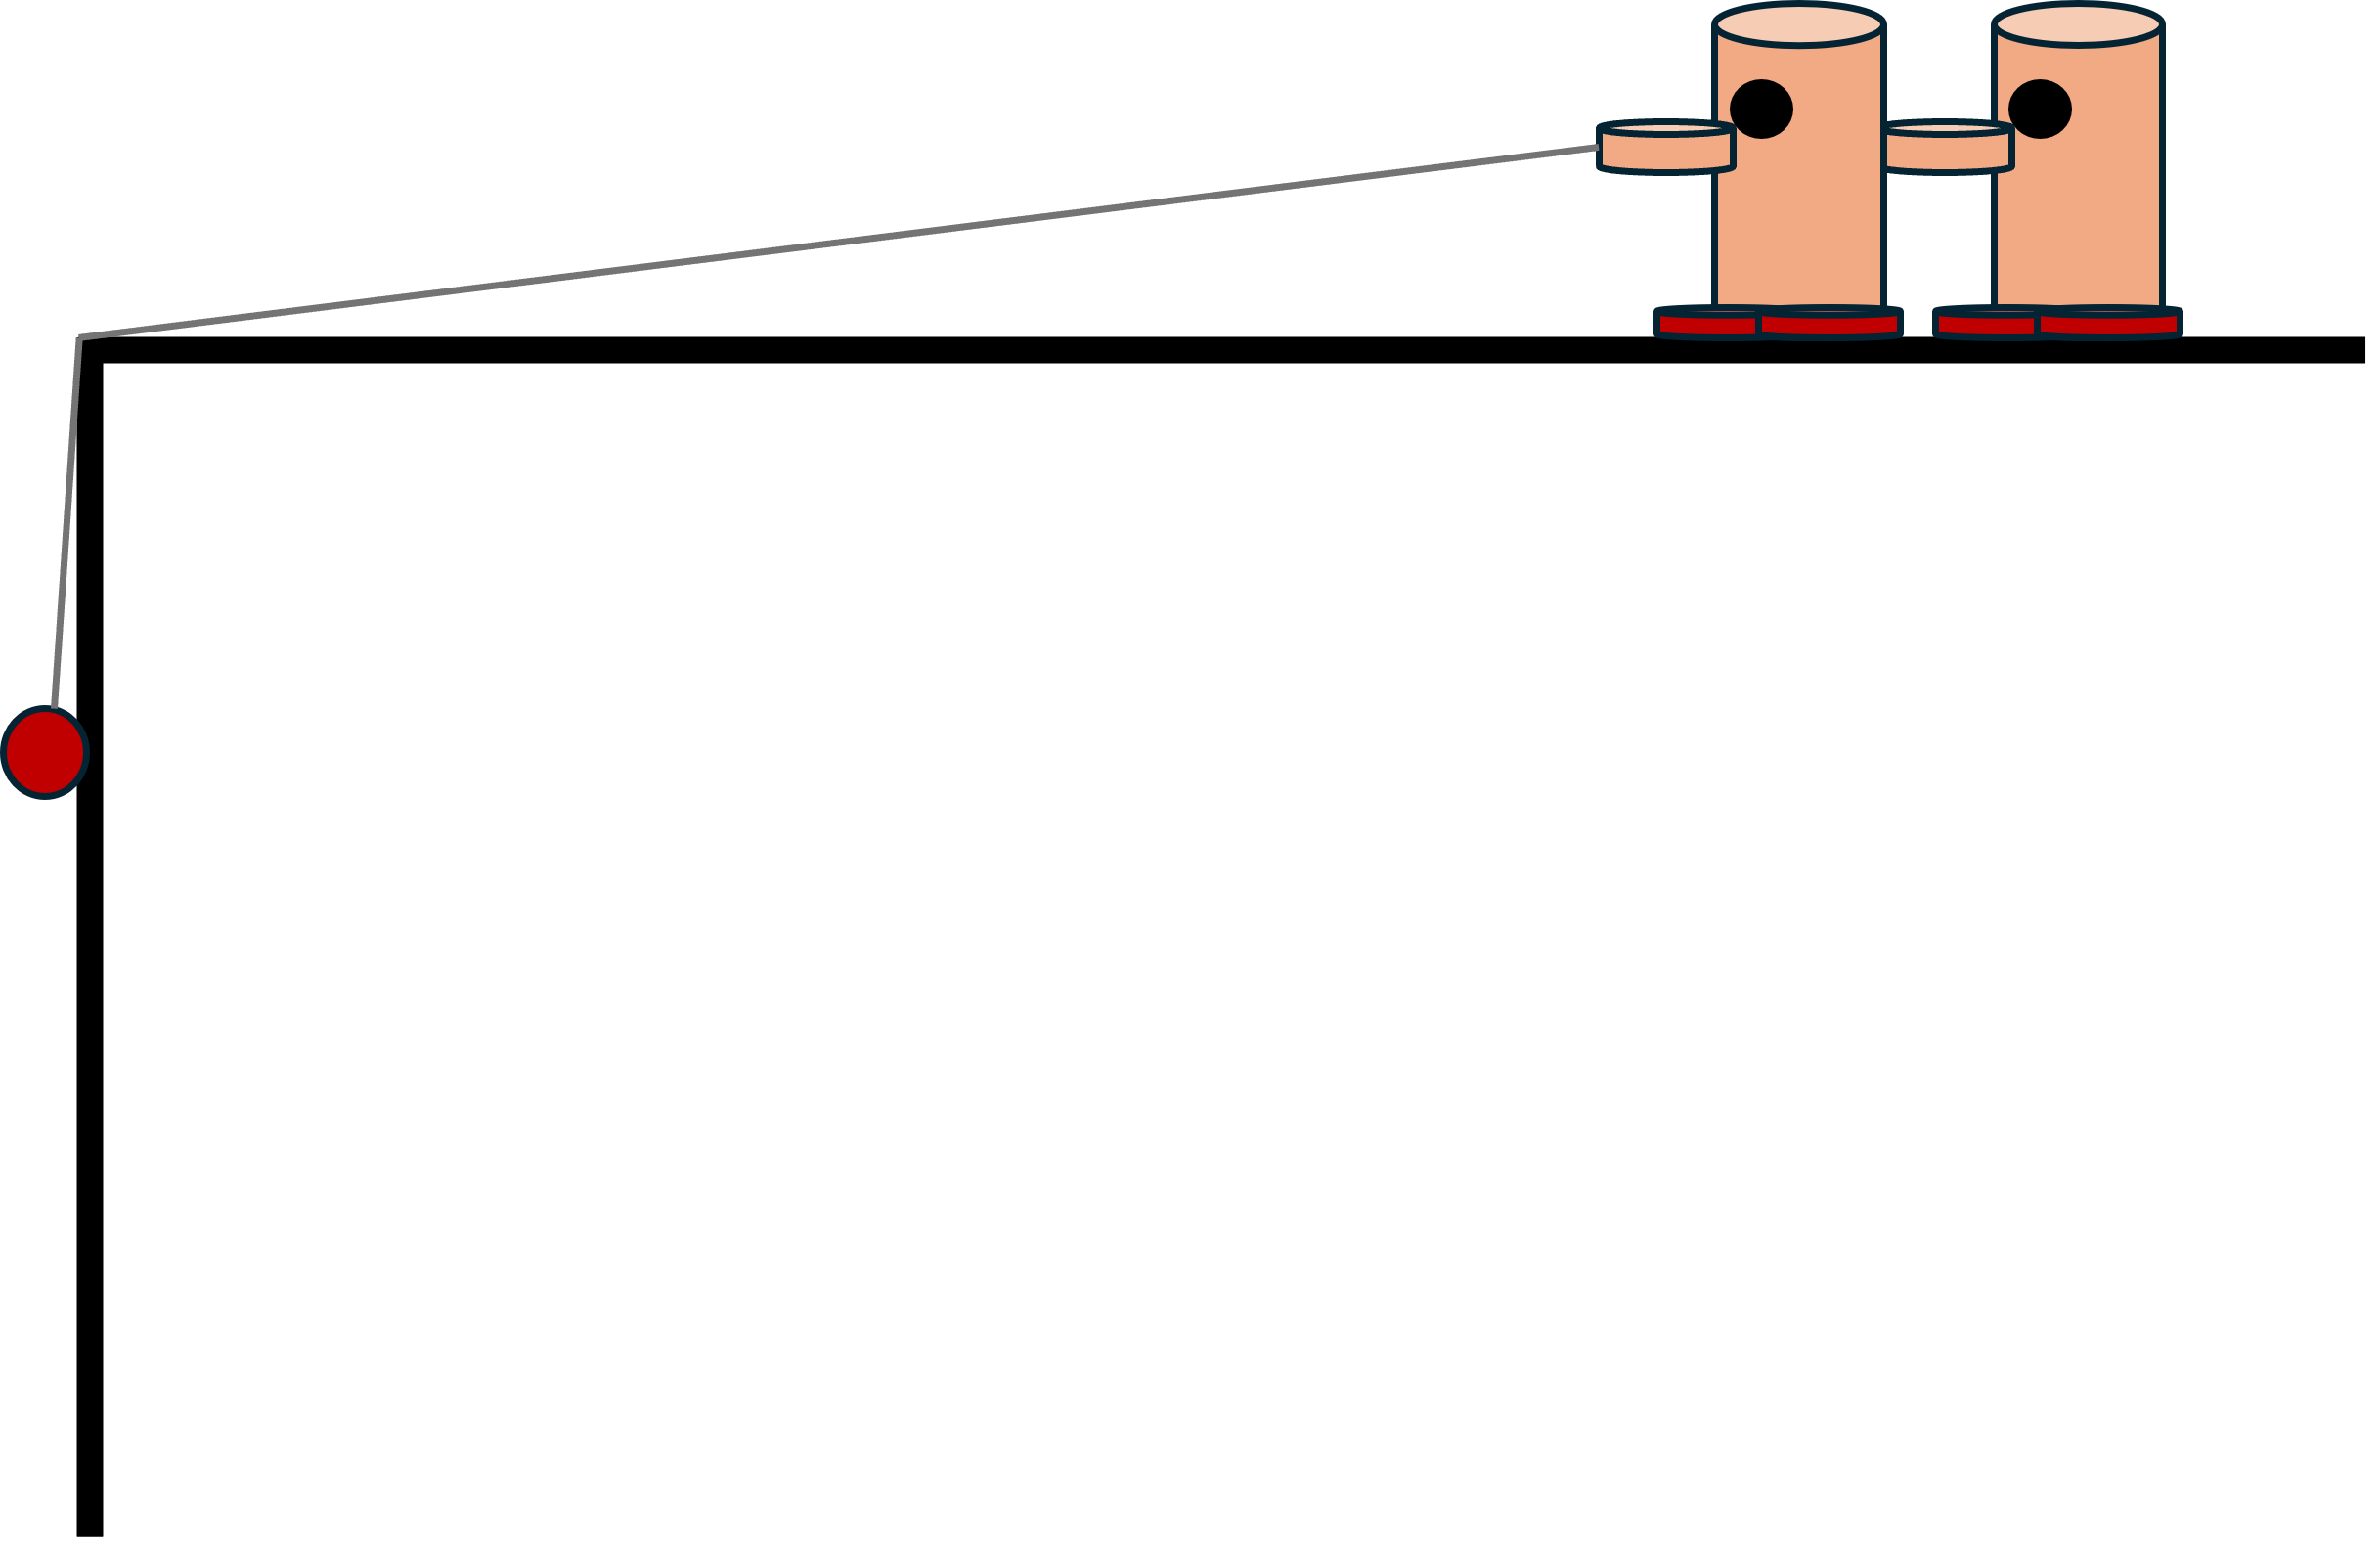
\includegraphics[width=11cm]{Bilder/männchen_kraftzerlegung_1.png}\\[0.3em]
{\small Bild 1: weit vom Rand entfernt, Seil verläuft flach}
\end{center}

\begin{center}
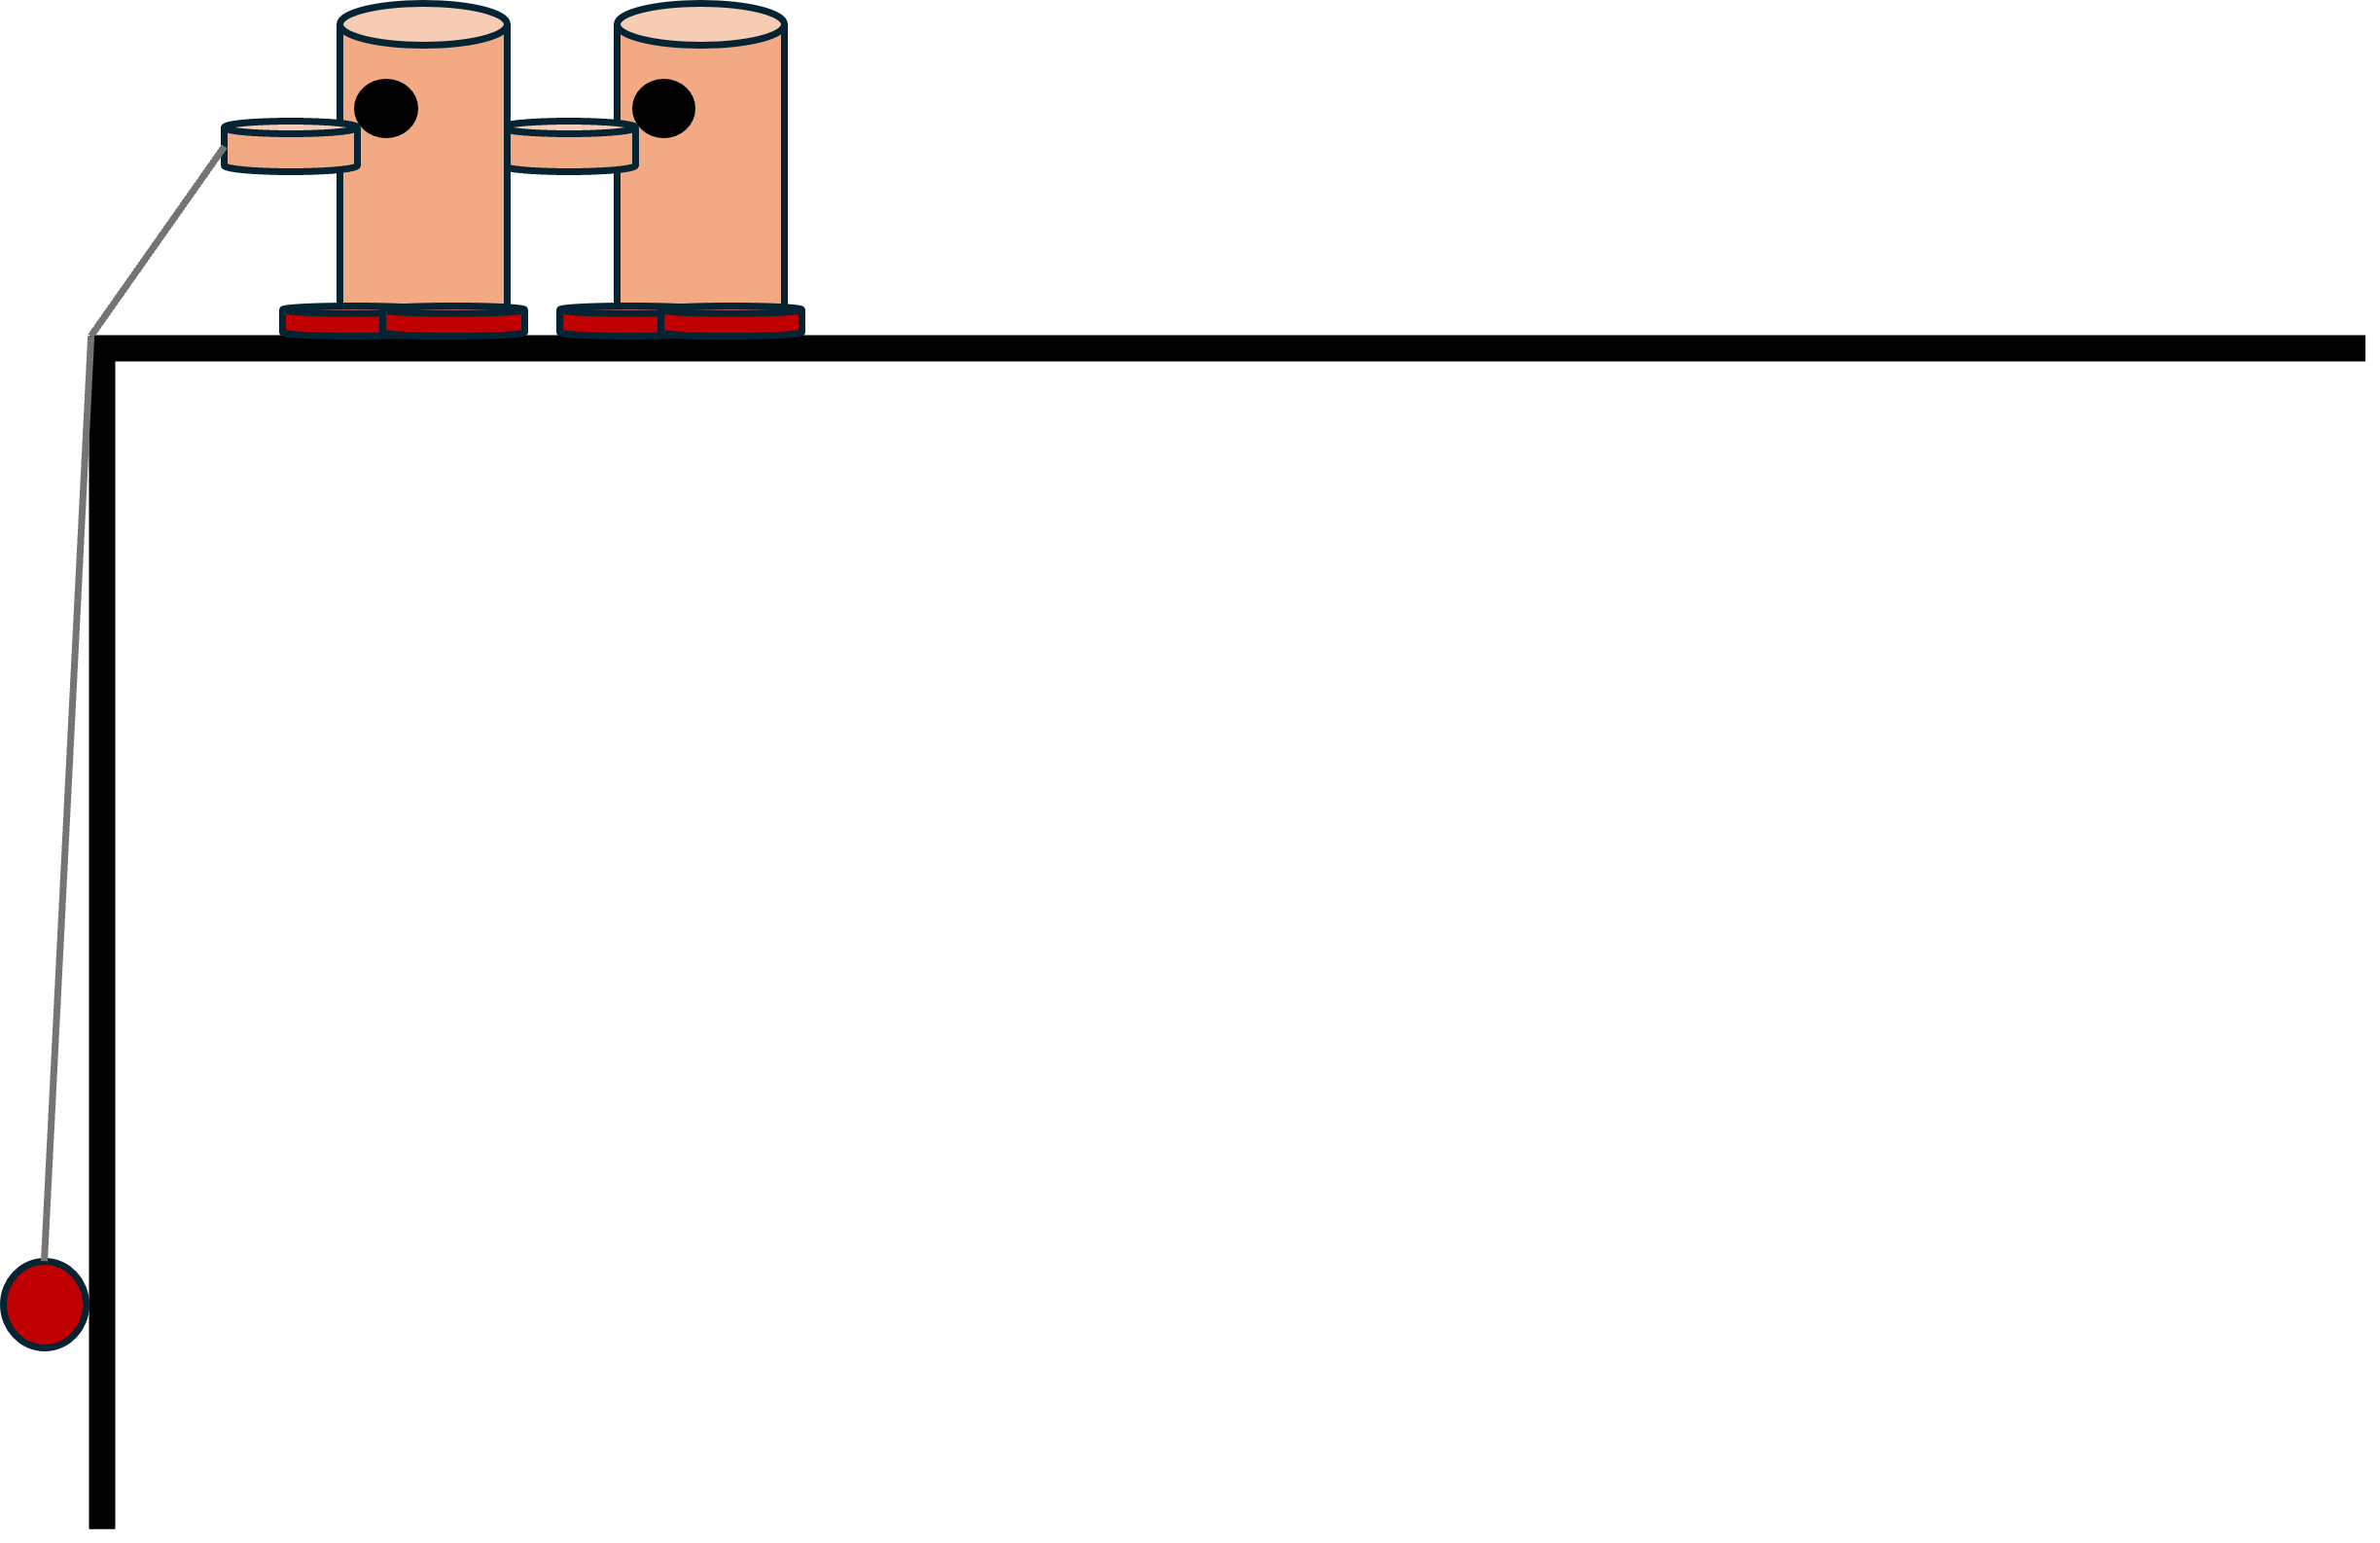
\includegraphics[width=11cm]{Bilder/männchen_kraftzerlegung_2.png}\\[0.3em]
{\small Bild 2: nah am Rand, Seil verläuft steil, Männchen stoppen}
\end{center}

\textbf{Erklärung:} Die Kraft im Seil (bestimmt durch die Gewichtskraft
des hängenden Gewichts) bleibt ungefähr gleich gross. Was sich ändert, ist
die Richtung, in der diese Kraft an der Nase zieht: Weit vom Tischrand
entfernt (Bild 1) verläuft das Seil von der Nase zur Tischkante fast
waagrecht: Die Kraft wirkt fast vollständig als horizontale Komponente,
die die Männchen nach vorne zieht. Je näher die Männchen dem Rand kommen
(Bild 2), desto steiler wird dieser Winkel: Die horizontale Komponente der
Kraft nimmt ab, während die vertikale Komponente (die eher an der Nase
nach oben zieht) zunimmt. Irgendwann reicht die verbleibende horizontale
Komponente nicht mehr aus, um die Männchen gegen die Reibung weiter nach
vorne zu ziehen. Sie bleiben kurz vor dem Rand stehen.

\end{document}
